\chapter{Testing}
\label{testing}
Dijkstra is often quoted as saying ``testing can only prove that errors are present, not that they are absent'' \cite{dijkstra}. This is true, but it is also the case that effective validation of a software product increases the confidence that a software product acts as it is supposed to.  This section of the dissertation is intended to convey information about the testing of the application, to increase the reader's confidence in the in the system and to convey information about the software engineering practice that was applied during testing.

\section{Unit Testing}
A unit test is a test on a unit of code in isolation: a comparison of the actual result of an operation with its expected output \cite{unitTesting}.  A series of unit tests can (and should) be run frequently to ensure that changes to code have not resulted in the development of problems elsewhere.  A unit test comprises of four main areas of execution:
\begin{enumerate}
	\item Set up -- the set up phase ensures that any prerequisites for the test are set up before the test begins, for example a session with a database;
	\item Act -- the phase where the unit of work under test is executed on the target object(s);
	\item Assert -- the comparison between the expected result and the actual result.  If the two do not match for a test (or an unexpected exception is thrown) it is said to have failed the test and if expected and actual results are the same, it is said to have passed;
	\item Tear down -- after each and every test, a tear down must occur.  Often, this is just a case of allowing the garbage collector to deal with unused objects, but sometimes connections to databases, file sessions and other connections must be closed.
\end{enumerate}

% NUnit - what, why, how.
NUnit is an open source unit testing framework for the .\gls{net} languages, originally ported from the unit testing framework for Java, JUnit \cite{nUnitHome}.  NUnit 2.5.7 is used within the project and was the most up-to-date version at the beginning of project development (released in August of 2010 \cite{nUnitRelease}).  

NUnit allows unit tests to be written as methods in a class, which can be run inside or outside the \gls{msvs} \gls{ide}, through ReSharper (see section \ref{devEnv}), which allows one-click running of unit tests and sets of unit tests.

\section{Continuous Integration}
\label{continuousIntegration}
Continuous Integration is a technique which minimises the risk of bugs cropping up between \gls{svn} revisions.  It works by automatically performing a build then running all unit tests each time a revision is committed to the repository, meaning that if issues arise between versions, they are noticed early and can be dealt with as and when they crop up.  There are several stages in setting up this process, as laid out by Martin Fowler in his paper on Continuous Integration \cite{fowlerCI}.  The important points are outlined below, but for the full approach (which is particularly aimed at teams of developers), see Fowler's article:
\begin{enumerate}
	\item A single source repository must be used.  This was achieved as laid out in section \ref{svn};
	\item The build must be automated.  This was achieved by bundling a command into a \gls{bat} script, which can in turn be run from the command line or the Windows Explorer interface.  This script used Microsoft's \texttt{msbuild} program, which uses an \gls{xml} file to organise how a build should take place, much like the way a \texttt{makefile} can be used in \gls{unix}-based operating systems;
	\item The build must be self-testing: tests are included as part of the \gls{xml} file mentioned in the previous step, which means that when the \gls{bat} file is run, all of the tests associated with the solution are executed on the freshly built executable.  This means that any bugs that crop up since the last build can be found and dealt with early, saving development and maintenance time later on;
	\item Every commit should build the mainline on an integration machine. In essence, this point is trying to ensure that the build and the test for the \gls{ci} cycle take place on a separate machine from the main development environment, ensuring that the project is not dependent on files left on the developer's machine --- in effect, this means that the \gls{ci} software must run on another computer.  This was achieved by using separate hardware from the developer machine, running \gls{ci} software called CruiseControl.NET (discussed below).  
	\item The developer is notified as soon as the build has finished, by way of a pop-up in the notification area of their computer.  Any issues can be fixed as soon as they arise, rather than being discovered further down the development line.
\end{enumerate}

CruiseControl.NET is an open-source program from Fowler's employer, ThoughtWorks, which acts as a monitor to the repository: it automatically checks-out code each time a commit takes place, builds the project and then runs all unit tests, before outputting the result of the build to both a web page and the CruiseControl Notification Tray client. \revisit - include screenshot of both

The \gls{ci} cycle is primarily intended for teams of developers. \gls{ci} leads to a `Test Early. Test Often. Test Automatically.' attitude --- it drives the developer to find find bugs now, which helps to avoid users finding bugs later \cite{pragmaticProgrammer}. Risks associated with deferred integration (integration after a long time or large numbers of changes, antonymous to continuous integration), which include .



CruiseControl.NET - what, why, how. Take from SE placement info to save time + effort \cite{fowlerCI}

\begin{figure}
	\begin{center}
		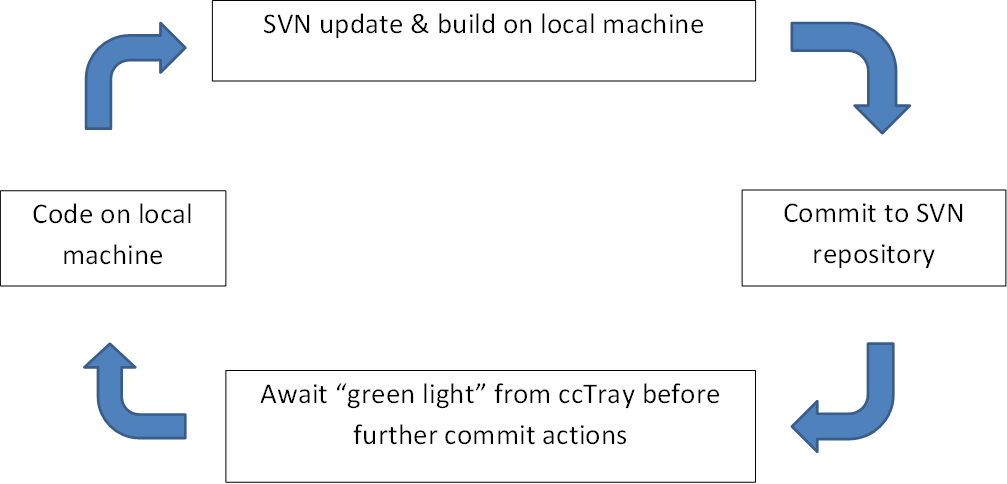
\includegraphics
			[scale=0.5]
			{images/ContinuousIntegration.png}
		\caption{The CI Cycle}
		\label{fig:continuousIntegration}
	\end{center}
\end{figure}

\section{Bug Tracking}
\label{bugTracking}
Bug tracking is, as the name suggests, the tracing of the status of bugs that have been discovered in a system, used primarily to ensure that bugs which are found are dealt with or logged in a release.  It is another concept that was encountered while on summer industrial placement, and it struck the developer as an advantageous \gls{case} tool to utilise in this project.

The bug tracker was used when a bug was encountered that was not going to be fixed at the time of the discovery; the developer wanted to apply use of the bug tracker intelligently so that it was always going to be a help, and not a bureaucratic hindrance to development.  Bugs that were found were created in the system and given a priority, marked initially as `open' to symbolise that they had not yet been dealt with.  When a bug had been dealt with and the developer had verified that it was no longer an issue, it was marked as `closed', and remained in the system for traceability, should a similar issue crop up.  As a rule of thumb, a comment was recorded to say firstly what the problem was, secondly what the fix was and thirdly which \gls{svn} (see section \ref{svn}) check-in fixed the issue so that one did not need to trawl through logs in \gls{svn} to find the fix, should they need to revisit it.\\ \revisit - want to check wording of this paragraph when I'm not tired.

The software used was BugTracker.NET -- a free, open-source, web-based bug tracker.  Having encountered this particular product and worked with it for three months, the developer thought it wise to stick to familiar ground and employ the same product.  The developer used hardware running at home to deploy BugTracker.NET and used it until a server failure in late January 2011.  As the hardware was no longer reliable to host the software, the decision was taken to switch bug tracking software to SourceForge's Bug tracker, which worked in a similar way.  Bugs from the old system (both open and closed) were transferred to the new site and remain there now for traceability and reference.

\section{Acceptance Test}
For the project to pass the acceptance test, all unit tests associated with the project must pass.  By the end of the project, there were \revisit unit tests, all of which passed.
